
The signal processing chain at the receiver are divided into four steps:
\begin{enumerate}
	\item Signal acquisition
	\item Signal tracking
	\begin{enumerate}
		\item Carrier Tracking
		\item Code Tracking
	\end{enumerate}
	\item Signal demodulation
	\item Channel decoding
\end{enumerate}
The signal processing part for NavIC signals at receiver are as shown in figure \ref{fig:demod_flow}.
\begin{normalsize}
	\begin{figure}[ht]
		\centering
		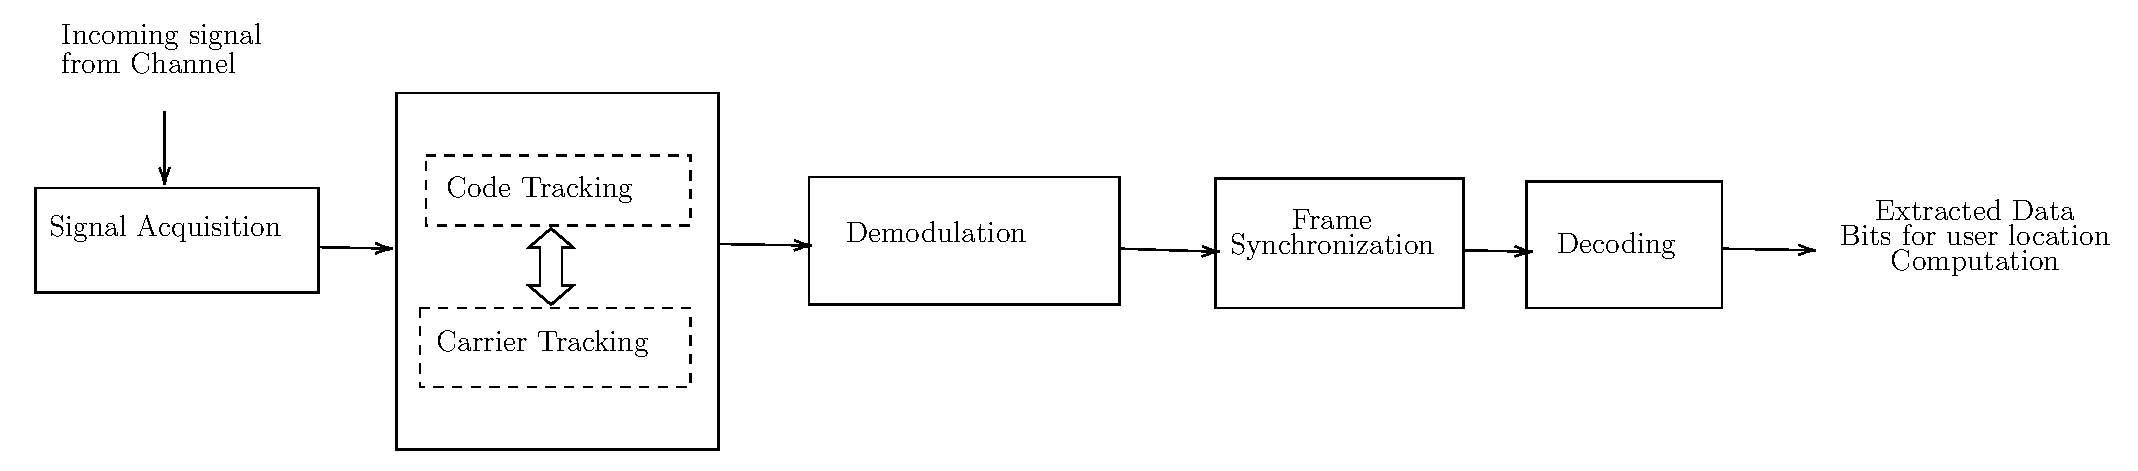
\includegraphics[width=1\columnwidth]{figs/receiver_block}
		\centering
		\captionsetup{justification=centering}
		\caption{The Block Level Architecture for Receiver}
		\label{fig:demod_flow}
	\end{figure}
\end{normalsize}
\\
\\
\begin{enumerate}
	\item \textbf{Signal acquisition:} The receiver searches for and acquires the NavIC signal for a given satellite(s) by correlating the received signal with a locally generated replica of the spreading code used by the satellite(s). This process helps in identifying the presence of the NavIC signal and estimating coarse value of both doppler frequency shift and code delay.
\item \textbf{Carrier tracking:} Once the signal is acquired, the receiver performs carrier tracking to estimate and track the carrier frequency and phase of the received signal. This is crucial for demodulation as it ensures accurate demodulation of the navigation message and ranging signal.
\item \textbf{Code delay tracking:} The receiver performs code delay tracking to estimate and track the spreading code used by the satellites. This helps in maintaining synchronization with the transmitted signal and extracting the navigation data and ranging information.

\item \textbf{Signal demodulation:}After the aquisition and tracking has been performed, the received data is mapped back using BPSK demodulation, mapping $-1$ to binary $1$ and $+1$ to binary $0$.
\item \textbf{Frame Synchronization:} The pilot PRN for every satellite is locally generated to determine the start of frame.
\item \textbf{Signal decoding:} Once the signal has been demodulated, the decoding is performed removing all the extra bits that were added to navigation data during the encoding process.
\end{enumerate}

\section{Signal Acquistion}
The role of the aqusition block is to examine the presence/absence of signals coming from a given satellite. In the case of signal being present, it should provide coarse estimations of the Code delay and the Carrier Doppler shift, yet accurate enough to initialize the frequency and code tracking loops.
\\
\\
A generic IRNSS signal defined by its complex baseband equivalent, 
$S_T(t)$, the digital signal at the input of an Acquisition block can be written as:
\begin{align}
	x_{IN}[k]=A(t)\hat s_T (t-\tau(t))e^{j(2 \pi f_D(t)t+\Phi(t))}\bigg|_{t=kT_s} +n(t)\bigg|_{t=kT_s}
\end{align}
\begin{table}[h]
%\centering
%%%%%%%%%%%%%%%%%%%%%%%%%%%%%%%%%%%%%%%%%%%%%%%%%%%%%%%%%%%%%%%%%%%%%%
%%                                                                  %%
%%  This is the header of a LaTeX2e file exported from Gnumeric.    %%
%%                                                                  %%
%%  This file can be compiled as it stands or included in another   %%
%%  LaTeX document. The table is based on the longtable package so  %%
%%  the longtable options (headers, footers...) can be set in the   %%
%%  preamble section below (see PRAMBLE).                           %%
%%                                                                  %%
%%  To include the file in another, the following two lines must be %%
%%  in the including file:                                          %%
%%        \def\inputGnumericTable{}                                 %%
%%  at the beginning of the file and:                               %%
%%        \input{name-of-this-file.tex}                             %%
%%  where the table is to be placed. Note also that the including   %%
%%  file must use the following packages for the table to be        %%
%%  rendered correctly:                                             %%
%%    \usepackage[latin1]{inputenc}                                 %%
%%    \usepackage{color}                                            %%
%%    \usepackage{array}                                            %%
%%    \usepackage{longtable}                                        %%
%%    \usepackage{calc}                                             %%
%%    \usepackage{multirow}                                         %%
%%    \usepackage{hhline}                                           %%
%%    \usepackage{ifthen}                                           %%
%%  optionally (for landscape tables embedded in another document): %%
%%    \usepackage{lscape}                                           %%
%%                                                                  %%
%%%%%%%%%%%%%%%%%%%%%%%%%%%%%%%%%%%%%%%%%%%%%%%%%%%%%%%%%%%%%%%%%%%%%%



%%  This section checks if we are begin input into another file or  %%
%%  the file will be compiled alone. First use a macro taken from   %%
%%  the TeXbook ex 7.7 (suggestion of Han-Wen Nienhuys).            %%
\def\ifundefined#1{\expandafter\ifx\csname#1\endcsname\relax}


%%  Check for the \def token for inputed files. If it is not        %%
%%  defined, the file will be processed as a standalone and the     %%
%%  preamble will be used.                                          %%
\ifundefined{inputGnumericTable}

%%  We must be able to close or not the document at the end.        %%
	\def\gnumericTableEnd{\end{document}}


%%%%%%%%%%%%%%%%%%%%%%%%%%%%%%%%%%%%%%%%%%%%%%%%%%%%%%%%%%%%%%%%%%%%%%
%%                                                                  %%
%%  This is the PREAMBLE. Change these values to get the right      %%
%%  paper size and other niceties.                                  %%
%%                                                                  %%
%%%%%%%%%%%%%%%%%%%%%%%%%%%%%%%%%%%%%%%%%%%%%%%%%%%%%%%%%%%%%%%%%%%%%%

	\documentclass[12pt%
			  %,landscape%
                    ]{report}
       \usepackage[latin1]{inputenc}
       \usepackage{fullpage}
       \usepackage{color}
       \usepackage{array}
       \usepackage{longtable}
       \usepackage{calc}
       \usepackage{multirow}
       \usepackage{hhline}
       \usepackage{ifthen}

	\begin{document}


%%  End of the preamble for the standalone. The next section is for %%
%%  documents which are included into other LaTeX2e files.          %%
\else

%%  We are not a stand alone document. For a regular table, we will %%
%%  have no preamble and only define the closing to mean nothing.   %%
    \def\gnumericTableEnd{}

%%  If we want landscape mode in an embedded document, comment out  %%
%%  the line above and uncomment the two below. The table will      %%
%%  begin on a new page and run in landscape mode.                  %%
%       \def\gnumericTableEnd{\end{landscape}}
%       \begin{landscape}


%%  End of the else clause for this file being \input.              %%
\fi

%%%%%%%%%%%%%%%%%%%%%%%%%%%%%%%%%%%%%%%%%%%%%%%%%%%%%%%%%%%%%%%%%%%%%%
%%                                                                  %%
%%  The rest is the gnumeric table, except for the closing          %%
%%  statement. Changes below will alter the table's appearance.     %%
%%                                                                  %%
%%%%%%%%%%%%%%%%%%%%%%%%%%%%%%%%%%%%%%%%%%%%%%%%%%%%%%%%%%%%%%%%%%%%%%

\providecommand{\gnumericmathit}[1]{#1} 
%%  Uncomment the next line if you would like your numbers to be in %%
%%  italics if they are italizised in the gnumeric table.           %%
%\renewcommand{\gnumericmathit}[1]{\mathit{#1}}
\providecommand{\gnumericPB}[1]%
{\let\gnumericTemp=\\#1\let\\=\gnumericTemp\hspace{0pt}}
 \ifundefined{gnumericTableWidthDefined}
        \newlength{\gnumericTableWidth}
        \newlength{\gnumericTableWidthComplete}
        \newlength{\gnumericMultiRowLength}
        \global\def\gnumericTableWidthDefined{}
 \fi
%% The following setting protects this code from babel shorthands.  %%
 \ifthenelse{\isundefined{\languageshorthands}}{}{\languageshorthands{english}}
%%  The default table format retains the relative column widths of  %%
%%  gnumeric. They can easily be changed to c, r or l. In that case %%
%%  you may want to comment out the next line and uncomment the one %%
%%  thereafter                                                      %%
\providecommand\gnumbox{\makebox[0pt]}
%%\providecommand\gnumbox[1][]{\makebox}

%% to adjust positions in multirow situations                       %%
\setlength{\bigstrutjot}{\jot}
\setlength{\extrarowheight}{\doublerulesep}

%%  The \setlongtables command keeps column widths the same across  %%
%%  pages. Simply comment out next line for varying column widths.  %%
\setlongtables

\setlength\gnumericTableWidth{%
	68pt+%
	235pt+%
0pt}
\def\gumericNumCols{2}
\setlength\gnumericTableWidthComplete{\gnumericTableWidth+%
         \tabcolsep*\gumericNumCols*2+\arrayrulewidth*\gumericNumCols}
\ifthenelse{\lengthtest{\gnumericTableWidthComplete > \linewidth}}%
         {\def\gnumericScale{\ratio{\linewidth-%
                        \tabcolsep*\gumericNumCols*2-%
                        \arrayrulewidth*\gumericNumCols}%
{\gnumericTableWidth}}}%
{\def\gnumericScale{1}}

%%%%%%%%%%%%%%%%%%%%%%%%%%%%%%%%%%%%%%%%%%%%%%%%%%%%%%%%%%%%%%%%%%%%%%
%%                                                                  %%
%% The following are the widths of the various columns. We are      %%
%% defining them here because then they are easier to change.       %%
%% Depending on the cell formats we may use them more than once.    %%
%%                                                                  %%
%%%%%%%%%%%%%%%%%%%%%%%%%%%%%%%%%%%%%%%%%%%%%%%%%%%%%%%%%%%%%%%%%%%%%%

\ifthenelse{\isundefined{\gnumericColA}}{\newlength{\gnumericColA}}{}\settowidth{\gnumericColA}{\begin{tabular}{@{}p{68pt*\gnumericScale}@{}}x\end{tabular}}
\ifthenelse{\isundefined{\gnumericColB}}{\newlength{\gnumericColB}}{}\settowidth{\gnumericColB}{\begin{tabular}{@{}p{235pt*\gnumericScale}@{}}x\end{tabular}}

\begin{longtable}[c]{%
	b{\gnumericColA}%
	b{\gnumericColB}%
	}

%%%%%%%%%%%%%%%%%%%%%%%%%%%%%%%%%%%%%%%%%%%%%%%%%%%%%%%%%%%%%%%%%%%%%%
%%  The longtable options. (Caption, headers... see Goosens, p.124) %%
%	\caption{The Table Caption.}             \\	%
% \hline	% Across the top of the table.
%%  The rest of these options are table rows which are placed on    %%
%%  the first, last or every page. Use \multicolumn if you want.    %%

%%  Header for the first page.                                      %%
%	\multicolumn{2}{c}{The First Header} \\ \hline 
%	\multicolumn{1}{c}{colTag}	%Column 1
%	&\multicolumn{1}{c}{colTag}	\\ \hline %Last column
%	\endfirsthead

%%  The running header definition.                                  %%
%	\hline
%	\multicolumn{2}{l}{\ldots\small\slshape continued} \\ \hline
%	\multicolumn{1}{c}{colTag}	%Column 1
%	&\multicolumn{1}{c}{colTag}	\\ \hline %Last column
%	\endhead

%%  The running footer definition.                                  %%
%	\hline
%	\multicolumn{2}{r}{\small\slshape continued\ldots} \\
%	\endfoot

%%  The ending footer definition.                                   %%
%	\multicolumn{2}{c}{That's all folks} \\ \hline 
%	\endlastfoot
%%%%%%%%%%%%%%%%%%%%%%%%%%%%%%%%%%%%%%%%%%%%%%%%%%%%%%%%%%%%%%%%%%%%%%

\hhline{|-|-}
	 \multicolumn{1}{|p{\gnumericColA}|}%
	{\gnumericPB{\raggedright}\gnumbox[l]{\hspace{0.75cm}\textbf{Symbol}}}
	&\multicolumn{1}{p{\gnumericColB}|}%
	{\gnumericPB{\raggedright}\gnumbox[l]{\hspace{3cm} \textbf{Definition}}}
\\
\hhline{|--|}
	 \multicolumn{1}{|p{\gnumericColA}|}%
	{\gnumericPB{\raggedright}\gnumbox[l]{\hspace{1cm}$x_{IN}[k]$}}
	&\multicolumn{1}{p{\gnumericColB}|}%
	{\gnumericPB{\raggedright}\gnumbox[l]{Complex vector $I,Q$ samples of received signal}}
\\
\hhline{|--|}
	 \multicolumn{1}{|p{\gnumericColA}|}%
	{\gnumericPB{\raggedright}\gnumbox[l]{\hspace{1cm}A(t)}}
	&\multicolumn{1}{p{\gnumericColB}|}%
	{\gnumericPB{\raggedright}\gnumbox[l]{Signal Amplitude}}
\\
\hhline{|--|}
	 \multicolumn{1}{|p{\gnumericColA}|}%
	{\gnumericPB{\raggedright}\gnumbox[l]{\hspace{1cm}$\hat s_T(t)$}}
	&\multicolumn{1}{p{\gnumericColB}|}%
	{\gnumericPB{\raggedright}\gnumbox[l]{filtered version of $s_T(t)$}}
\\
\hhline{|--|}
	 \multicolumn{1}{|p{\gnumericColA}|}%
	{\gnumericPB{\raggedright}\gnumbox[l]{\hspace{1cm}$f_D(t)$ }}
	&\multicolumn{1}{p{\gnumericColB}|}%
	{\gnumericPB{\raggedright}\gnumbox[l]{Time varying doppler shift}}
\\
\hhline{|--|}
	 \multicolumn{1}{|p{\gnumericColA}|}%
	{\gnumericPB{\raggedright}\gnumbox[l]{\hspace{1cm}$\Phi (t)$}}
	&\multicolumn{1}{p{\gnumericColB}|}%
	{\gnumericPB{\raggedright}\gnumbox[l]{Time varying carrier phase shift}}
\\
\hhline{|--|}
	 \multicolumn{1}{|p{\gnumericColA}|}%
	{\gnumericPB{\raggedright}\gnumbox[l]{\hspace{1cm}$\tau (t)$}}
	&\multicolumn{1}{p{\gnumericColB}|}%
	{\gnumericPB{\raggedright}\gnumbox[l]{Time varying code delay}}
\\
\hhline{|--|}
	 \multicolumn{1}{|p{\gnumericColA}|}%
	{\gnumericPB{\raggedright}\gnumbox[l]{\hspace{1cm}n(t) }}
	&\multicolumn{1}{p{\gnumericColB}|}%
	{\gnumericPB{\raggedright}\gnumbox[l]{Time varying random noise}}
\\
\hhline{|--|}
	 \multicolumn{1}{|p{\gnumericColA}|}%
	{\gnumericPB{\raggedright}\gnumbox[l]{\hspace{1cm}$T_s$ }}
	&\multicolumn{1}{p{\gnumericColB}|}%
	{\gnumericPB{\raggedright}\gnumbox[l]{Sampling period}}
\\
\hhline{|-|-|}
\end{longtable}

\ifthenelse{\isundefined{\languageshorthands}}{}{\languageshorthands{\languagename}}
\gnumericTableEnd

\vspace{3mm}
\caption{Parameters Table in Signal Acquisition}
\label{table:table_para}
\end{table}

\subsection{Implementation of CA PCPS Acquisition}
The Parallel Code Phase Search (PCPS) algorithm is used in Acquisition block and is depicted in figure \ref{fig:pcps_flow} and described as follows:
\begin{normalsize}
\begin{figure}[ht]
	\centering
	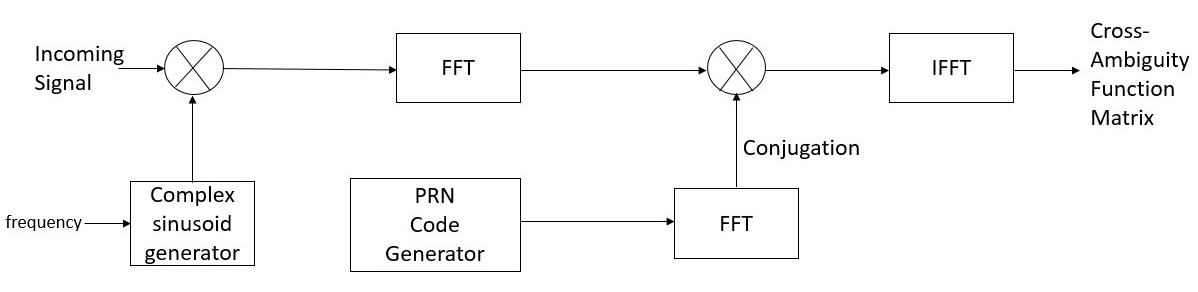
\includegraphics[width=1\columnwidth]{figs/pcps}
	\centering
	\captionsetup{justification=centering}
	\caption{PCPS algorithm flow}
	\label{fig:pcps_flow}
\end{figure}
\end{normalsize}
\\
\textbf{Given:}
\begin{enumerate}
	\item Input signal buffer $x_{IN}$ of K complex samples, provided by the Signal Conditioner 
	\item On-memory FFT of the local replica
	\begin{align}
		D[k]=FFT_K\{d[k]\}
	\end{align}
	\item Acquisition threshold  $\gamma$
	\item Frequency span : \sbrak{f_{min}, f_{max}}
	\item Frequency step : $f_{step}$
\end{enumerate}
\textbf{Expected:}
\begin{enumerate}
	\item Find out if signal is acquired or not for a given satellite(s) 
	\item If signal is acquired, for each given satellite, calculate coarse estimation of Doppler shift $\hat f_{D_{acq}}$ and Code delay $\hat \tau_{acq}$
\end{enumerate}
\textbf{Algorithm:}
\begin{enumerate}
	\item Calculate input signal power estimation  $\hat P_{in} = \frac{1}{K}\sum_{k=0}^{K-1} \big| x_{IN}[k]\big| ^2$
	\item for $\check f_D=[ f_{min} to f_{max}]\text{ in }f_{steps}$ 
	\begin{enumerate}
		\item Calculate carrier wipe off$\hspace{0.5cm}x[k]=x_{IN}[k]e^{-(j2 \pi \check f_D k T_s)}$,for $k=0,...,K-1$
		\item Calculate $X[k]=FFT_K\{x[k]\}$
		\item Calculate $Y[k]=X[k].D[k]$, for $k=0,...K-1$ 
        	\item Calculate corresponding column in the Cross ambiguity function matrix - $R_{xd}(\check f_D,\tau) = \frac{1}{K^2}IFFT_K\{Y[k]\}$
        \end{enumerate}

        \item Search maximum and its indices in the search grid:
	\begin{align}
		\{S_{max},f_i,\tau_j\} = max_{f,\tau} \big |R_{xd}(f,\tau)\big | ^2
	\end{align}
        \item	Calculate the Generalized Likelihood Ratio Test (GLRT) function with normalized variance:
	\begin{align}
		\Gamma_{GLRT} = \frac{2KS_{max}}{\hat P_{in}}
	\end{align}
	\item if $\Gamma_{GLRT} > \gamma$\\
	Declare positive acquisition and provides coarse estimation of code delay $\hat \tau_{acq} = \tau_j $ and Doppler shift $\hat f_{D_{acq}}=f_i$,\\
	other wise declare negative acquisition.\\
\end{enumerate}


\section{Tracking}
The role of tracking block is to follow signal synchronization parameters: code phase, Doppler shift and carrier phase and extract the baseband signal. It performs the following 3 function to decipher the baseband signal from the incoming signal as shown in figure \ref{fig:tracking}. 
\begin{enumerate}
	\item Carrier and code wipeoff 
	\item Pre-detection integration
	\item Baseband signal processing
\end{enumerate}

\begin{normalsize}
\begin{figure}[ht]
\centering
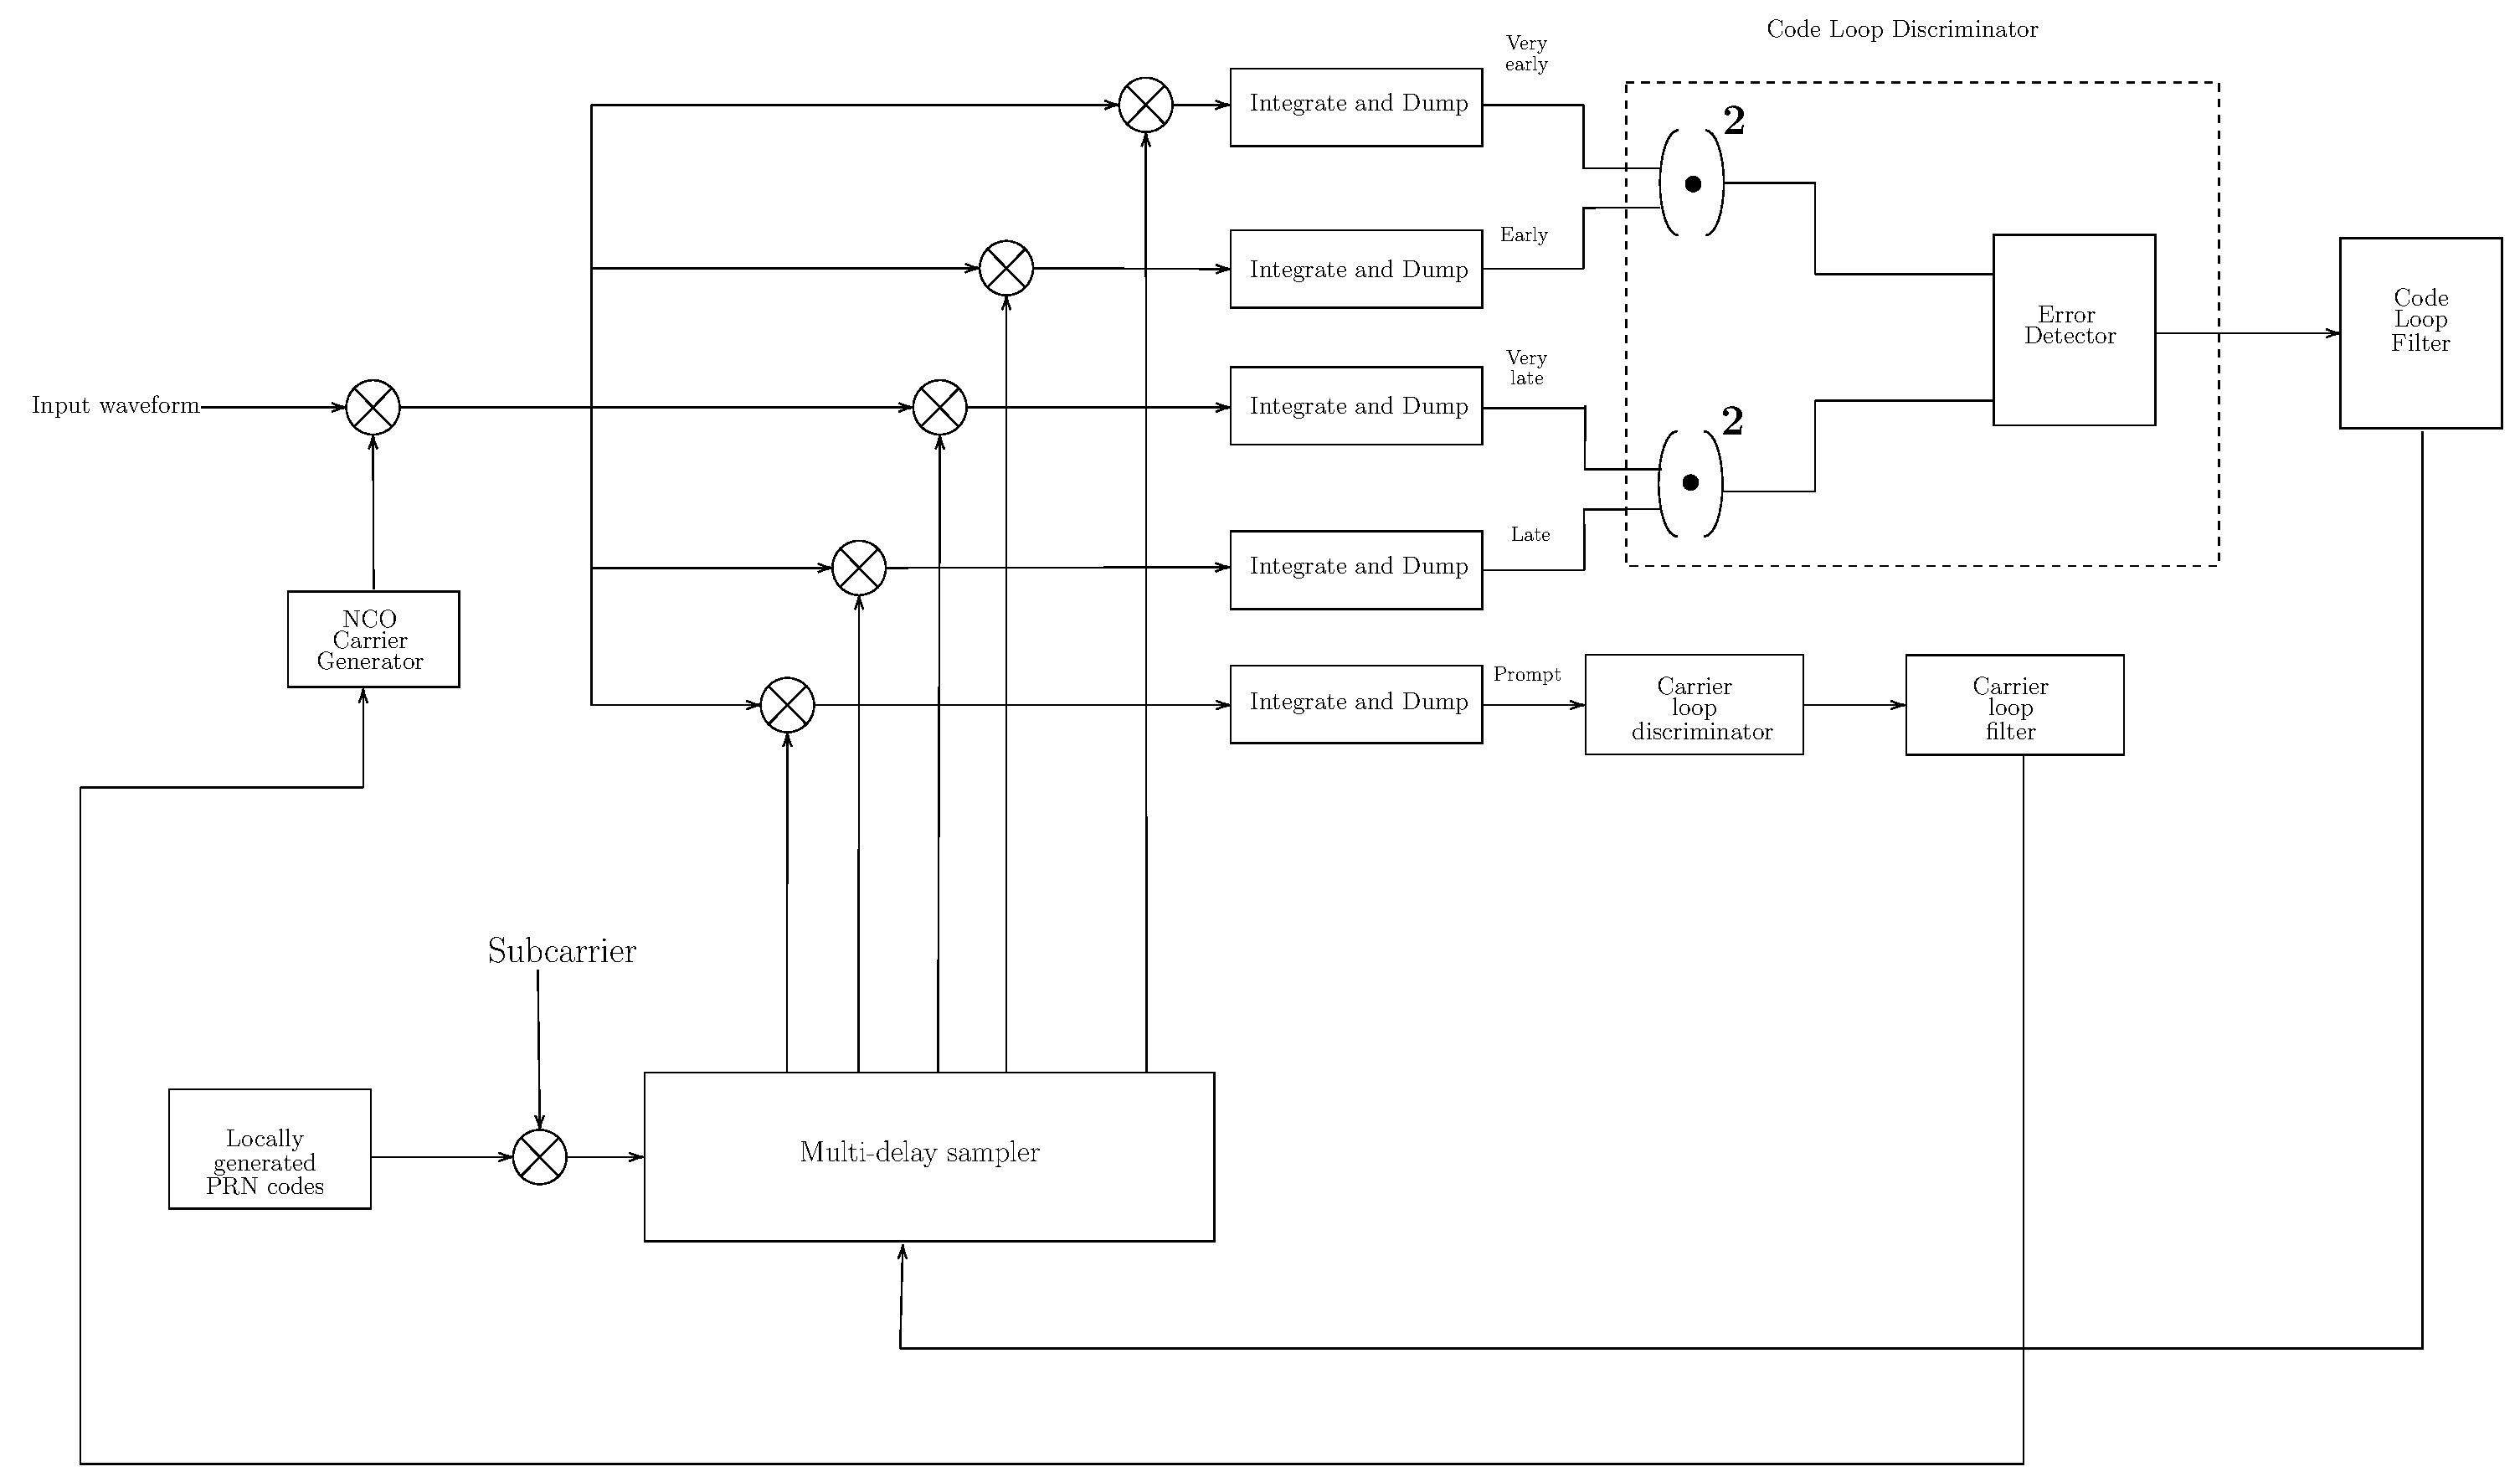
\includegraphics[width=1.25\columnwidth]{figs/tracking}
\centering
\captionsetup{justification=centering}
\caption{Tracking block diagram}
\label{fig:tracking}
\end{figure}
\end{normalsize}
\subsection{Carrier and code wipeoff}
\textbf{Carrier wipeoff: }Referring to the figure \ref{fig:tracking}, first the incoming signal is stripped off the carrier (plus carrier Doppler) by the replica carrier (plus carrier Doppler) signals. The replica carrier (including carrier Doppler) signals are synthesized by the carrier numerically controlled oscillator (NCO). In closed loop operation, the carrier NCO is controlled by the carrier tracking loop in the receiver processor.
\\
\textbf{Code wipeoff: } The received signal is then correlated with very early(VE), early(E), prompt(P), late(L) and very late(VL) replica codes (plus code Doppler) synthesized by a multi-delay sampler. In the closed loop operation, the code NCO is controlled by the code tracking loop in the receiver processor. E and L are typically separated in phase by 0.3 chips and P is in the middle. VE and VL are separated by 1.2 chips. The prompt replica code phase is aligned with the incoming satellite code phase producing maximum correlation if it is tracking the incoming satellite code phase. Under this circumstance, the early phase is aligned a fraction of a chip period early, and the late phase is aligned the same fraction of the chip period late with respect to the incoming  code phase, and these correlators produce about half the maximum correlation. Any misalignment in the replica code phase with respect to the incoming code phase produces a difference in the vector magnitudes of the early and late correlated outputs so that the amount and direction of the phase change can be detected and corrected by the code tracking loop.
\subsection{Pre-detection and integration}
Extensive digital predetection integration and dump processes occur after the carrier and code wiping off processes. Figure \ref{fig:tracking} shows five complex correlators required to produce five
components, which are integrated and dumped to produce very early, early, prompt, late and very late vesions of the signal . The carrier wipeoff and code wipeoff processes must be performed at the digital IF sample rate, while the integrate and dump accumulators provide filtering and resampling at the processor baseband input rate, which can be at 1,000 Hz during search modes or as low as 50 Hz during
track modes, depending on the desired dwell time during search or the desired predetection integration time during track.
\subsection{Baseband signal processing}
This entails Carrier tracking and Code tracking using Phase locked loop (PLL), Frequency locked loop (FLL) and Delay locked loop (DLL). 


\subsubsection{Carrier tracking loop}
\textbf{Phase locked loop(PLL)}\\
The carrier loop discriminator defines the type of tracking loop as a PLL, a Costas PLL (which is a PLL-type discriminator that tolerates the presence of data modulation on the baseband signal), or a frequency lock loop (FLL). Carrier tracking loop tracks the frequency and phase of the received signal by detecting the phase error between replicated signal and incoming signal and accordingly replicated signal produced by numerically controlled oscillator (NCO) is adjusted to synchronize with incoming signal in both frequency and phase. For zero phase error detected, navigation data is accurately extracted. 
\begin{align}
  %\text{Phase error} =ATAN2(I_P,Q_P) = \tan^{-1}\brak{\frac{I_P}{Q_P}}
  \text{Phase error}_{pilot} &=ATAN2(I_P,Q_P) = \tan^{-1}\brak{\frac{I_P}{Q_P}}\\
  \text{Phase error}_{data} &=ATAN2(Q_P,I_P) = \tan^{-1}\brak{\frac{Q_P}{I_P}}
\end{align}
The ATAN2 discriminator is the only one that remains linear over the full input error range of $\pm180^{\circ}$. However, in the presence of noise, both of the discriminator outputs are linear only near the $0^{\circ}$ region. These PLL discriminators will achieve the 6-dB improvement in signal tracking threshold (by comparison with the Costas discriminators) for the dataless carrier because they track the full four quadrant range of the input signal.
\\
\\
\textbf{Frequency locked loop}\\
PLLs replicate the exact phase and frequency of the incoming SV (converted to IF) to perform the carrier wipeoff function. FLLs perform the carrier wipeoff process by replicating the approximate frequency, and they typically permit the phase to rotate with respect to the incoming carrier signal. The algorithm used in FLL discriminator is $\frac{\text{ATAN2}{\brak{cross,dot}}}{t_2-t_1}$. The frequency error is given by 
\begin{align}
	\text{Frequency error} = \frac{\phi_2-\phi_1}{t_2-t_1}
\end{align}

\noindent The phase change $\phi_2 - \phi_1$ between two adjacent samples of $I_{PS}$ and $Q_{PS}$ at times $t_2$ and $t_1$ is computed. This phase change in a fixed interval of time is proportinal to frequenct error in the carrier tracking loop. The error is fed to carier NCO to adjust the frequency to lock to the right frequency.

\subsubsection{Code tracking loop}
\textbf{Delay locked loop:}
Post the carrier signal synchronization, received CA code samples are synchronized by aligning with replicated CA code samples by shifting right or left. To determine the direction of shift, the I and Q outputs are multiplied with prompt code (PRN code which is phase aligned), early code (prompt PRN code shifted by some samples to the right) and late code (prompt PRN code shifted by some samples to the left) resulting in corresponding to I and Q channel respectively. Following algorithm is used to lock the code phase.

\begin{align}
	E_K&=\sqrt[]{VE^2+E^2}\\
	L_K&=\sqrt[]{VL^2+L^2}
\end{align}

\begin{align}
	\text{DLL Discriminator} (\epsilon)&=\frac{1}{2}\frac{E_K-L_K}{E_K+L_K}
\end{align}

\noindent If the replica code is aligned, then the early and late envelopes are equal in amplitude and no error is generated by the discriminator. If the replica code is misaligned, then the early and late envelopes are unequal by an amount that is proportional to the amount of code phase error between the replica and the incoming signal (within the limits of the correlation interval). The code discriminator senses the amount of error in the replica code and the direction (early or late) from the difference in the amplitudes of the early and late envelopes. This
error is filtered and then applied to the code loop NCO, where the output code shift is increased or decreased as necessary to correct the replica code generator phase with respect to the incoming SV signal code phase.

\subsubsection{Loop filter characteristics}
\begin{table}[h]
%\centering
%%%%%%%%%%%%%%%%%%%%%%%%%%%%%%%%%%%%%%%%%%%%%%%%%%%%%%%%%%%%%%%%%%%%%%
%%                                                                  %%
%%  This is the header of a LaTeX2e file exported from Gnumeric.    %%
%%                                                                  %%
%%  This file can be compiled as it stands or included in another   %%
%%  LaTeX document. The table is based on the longtable package so  %%
%%  the longtable options (headers, footers...) can be set in the   %%
%%  preamble section below (see PRAMBLE).                           %%
%%                                                                  %%
%%  To include the file in another, the following two lines must be %%
%%  in the including file:                                          %%
%%        \def\inputGnumericTable{}                                 %%
%%  at the beginning of the file and:                               %%
%%        \input{name-of-this-file.tex}                             %%
%%  where the table is to be placed. Note also that the including   %%
%%  file must use the following packages for the table to be        %%
%%  rendered correctly:                                             %%
%%    \usepackage[latin1]{inputenc}                                 %%
%%    \usepackage{color}                                            %%
%%    \usepackage{array}                                            %%
%%    \usepackage{longtable}                                        %%
%%    \usepackage{calc}                                             %%
%%    \usepackage{multirow}                                         %%
%%    \usepackage{hhline}                                           %%
%%    \usepackage{ifthen}                                           %%
%%  optionally (for landscape tables embedded in another document): %%
%%    \usepackage{lscape}                                           %%
%%                                                                  %%
%%%%%%%%%%%%%%%%%%%%%%%%%%%%%%%%%%%%%%%%%%%%%%%%%%%%%%%%%%%%%%%%%%%%%%



%%  This section checks if we are begin input into another file or  %%
%%  the file will be compiled alone. First use a macro taken from   %%
%%  the TeXbook ex 7.7 (suggestion of Han-Wen Nienhuys).            %%
\def\ifundefined#1{\expandafter\ifx\csname#1\endcsname\relax}


%%  Check for the \def token for inputed files. If it is not        %%
%%  defined, the file will be processed as a standalone and the     %%
%%  preamble will be used.                                          %%
\ifundefined{inputGnumericTable}

%%  We must be able to close or not the document at the end.        %%
	\def\gnumericTableEnd{\end{document}}


%%%%%%%%%%%%%%%%%%%%%%%%%%%%%%%%%%%%%%%%%%%%%%%%%%%%%%%%%%%%%%%%%%%%%%
%%                                                                  %%
%%  This is the PREAMBLE. Change these values to get the right      %%
%%  paper size and other niceties.                                  %%
%%                                                                  %%
%%%%%%%%%%%%%%%%%%%%%%%%%%%%%%%%%%%%%%%%%%%%%%%%%%%%%%%%%%%%%%%%%%%%%%

	\documentclass[12pt%
			  %,landscape%
                    ]{report}
       \usepackage[latin1]{inputenc}
       \usepackage{fullpage}
       \usepackage{color}
       \usepackage{array}
       \usepackage{longtable}
       \usepackage{calc}
       \usepackage{multirow}
       \usepackage{hhline}
       \usepackage{ifthen}

	\begin{document}


%%  End of the preamble for the standalone. The next section is for %%
%%  documents which are included into other LaTeX2e files.          %%
\else

%%  We are not a stand alone document. For a regular table, we will %%
%%  have no preamble and only define the closing to mean nothing.   %%
    \def\gnumericTableEnd{}

%%  If we want landscape mode in an embedded document, comment out  %%
%%  the line above and uncomment the two below. The table will      %%
%%  begin on a new page and run in landscape mode.                  %%
%       \def\gnumericTableEnd{\end{landscape}}
%       \begin{landscape}


%%  End of the else clause for this file being \input.              %%
\fi

%%%%%%%%%%%%%%%%%%%%%%%%%%%%%%%%%%%%%%%%%%%%%%%%%%%%%%%%%%%%%%%%%%%%%%
%%                                                                  %%
%%  The rest is the gnumeric table, except for the closing          %%
%%  statement. Changes below will alter the table's appearance.     %%
%%                                                                  %%
%%%%%%%%%%%%%%%%%%%%%%%%%%%%%%%%%%%%%%%%%%%%%%%%%%%%%%%%%%%%%%%%%%%%%%

\providecommand{\gnumericmathit}[1]{#1} 
%%  Uncomment the next line if you would like your numbers to be in %%
%%  italics if they are italizised in the gnumeric table.           %%
%\renewcommand{\gnumericmathit}[1]{\mathit{#1}}
\providecommand{\gnumericPB}[1]%
{\let\gnumericTemp=\\#1\let\\=\gnumericTemp\hspace{0pt}}
 \ifundefined{gnumericTableWidthDefined}
        \newlength{\gnumericTableWidth}
        \newlength{\gnumericTableWidthComplete}
        \newlength{\gnumericMultiRowLength}
        \global\def\gnumericTableWidthDefined{}
 \fi
%% The following setting protects this code from babel shorthands.  %%
 \ifthenelse{\isundefined{\languageshorthands}}{}{\languageshorthands{english}}
%%  The default table format retains the relative column widths of  %%
%%  gnumeric. They can easily be changed to c, r or l. In that case %%
%%  you may want to comment out the next line and uncomment the one %%
%%  thereafter                                                      %%
\providecommand\gnumbox{\makebox[0pt]}
%%\providecommand\gnumbox[1][]{\makebox}

%% to adjust positions in multirow situations                       %%
\setlength{\bigstrutjot}{\jot}
\setlength{\extrarowheight}{\doublerulesep}

%%  The \setlongtables command keeps column widths the same across  %%
%%  pages. Simply comment out next line for varying column widths.  %%
\setlongtables

\setlength\gnumericTableWidth{%
	70pt+%
	100pt+%
	80pt+%
0pt}
\def\gumericNumCols{3}
\setlength\gnumericTableWidthComplete{\gnumericTableWidth+%
         \tabcolsep*\gumericNumCols*2+\arrayrulewidth*\gumericNumCols}
\ifthenelse{\lengthtest{\gnumericTableWidthComplete > \linewidth}}%
         {\def\gnumericScale{\ratio{\linewidth-%
                        \tabcolsep*\gumericNumCols*2-%
                        \arrayrulewidth*\gumericNumCols}%
{\gnumericTableWidth}}}%
{\def\gnumericScale{1}}

%%%%%%%%%%%%%%%%%%%%%%%%%%%%%%%%%%%%%%%%%%%%%%%%%%%%%%%%%%%%%%%%%%%%%%
%%                                                                  %%
%% The following are the widths of the various columns. We are      %%
%% defining them here because then they are easier to change.       %%
%% Depending on the cell formats we may use them more than once.    %%
%%                                                                  %%
%%%%%%%%%%%%%%%%%%%%%%%%%%%%%%%%%%%%%%%%%%%%%%%%%%%%%%%%%%%%%%%%%%%%%%

\ifthenelse{\isundefined{\gnumericColA}}{\newlength{\gnumericColA}}{}\settowidth{\gnumericColA}{\begin{tabular}{@{}p{70pt*\gnumericScale}@{}}x\end{tabular}}
\ifthenelse{\isundefined{\gnumericColB}}{\newlength{\gnumericColB}}{}\settowidth{\gnumericColB}{\begin{tabular}{@{}p{100pt*\gnumericScale}@{}}x\end{tabular}}
\ifthenelse{\isundefined{\gnumericColC}}{\newlength{\gnumericColC}}{}\settowidth{\gnumericColC}{\begin{tabular}{@{}p{80pt*\gnumericScale}@{}}x\end{tabular}}

\begin{longtable}[c]{%
	b{\gnumericColA}%
	b{\gnumericColB}%
	b{\gnumericColC}%
	}

%%%%%%%%%%%%%%%%%%%%%%%%%%%%%%%%%%%%%%%%%%%%%%%%%%%%%%%%%%%%%%%%%%%%%%
%%  The longtable options. (Caption, headers... see Goosens, p.124) %%
%	\caption{The Table Caption.}             \\	%
% \hline	% Across the top of the table.
%%  The rest of these options are table rows which are placed on    %%
%%  the first, last or every page. Use \multicolumn if you want.    %%

%%  Header for the first page.                                      %%
%	\multicolumn{3}{c}{The First Header} \\ \hline 
%	\multicolumn{1}{c}{colTag}	%Column 1
%	&\multicolumn{1}{c}{colTag}	%Column 2
%	&\multicolumn{1}{c}{colTag}	\\ \hline %Last column
%	\endfirsthead

%%  The running header definition.                                  %%
%	\hline
%	\multicolumn{3}{l}{\ldots\small\slshape continued} \\ \hline
%	\multicolumn{1}{c}{colTag}	%Column 1
%	&\multicolumn{1}{c}{colTag}	%Column 2
%	&\multicolumn{1}{c}{colTag}	\\ \hline %Last column
%	\endhead

%%  The running footer definition.                                  %%
%	\hline
%	\multicolumn{3}{r}{\small\slshape continued\ldots} \\
%	\endfoot

%%  The ending footer definition.                                   %%
%	\multicolumn{3}{c}{That's all folks} \\ \hline 
%	\endlastfoot
%%%%%%%%%%%%%%%%%%%%%%%%%%%%%%%%%%%%%%%%%%%%%%%%%%%%%%%%%%%%%%%%%%%%%%

\hhline{|-|-|-}
	 \multicolumn{1}{|p{\gnumericColA}|}%
	{\gnumericPB{\raggedright}\gnumbox[l]{\textbf{Loop Order}}}
	&\multicolumn{1}{p{\gnumericColB}|}%
	{\gnumericPB{\raggedright}\gnumbox[l]{\textbf{Noise Bandwidth}}}
	&\multicolumn{1}{p{\gnumericColC}|}%
	{\gnumericPB{\raggedright}\gnumbox[l]{\textbf{Typical Filter  }}}
\\
%\hhline{|---|}
	 \multicolumn{1}{|p{\gnumericColA}|}%
	{\gnumericPB{\raggedleft}\gnumbox[r]{}}
	&\multicolumn{1}{p{\gnumericColB}|}%
	{\gnumericPB{\raggedright}\gnumbox[l]{\textbf{$ B_n$ (Hz)}}}
	&\multicolumn{1}{p{\gnumericColC}|}%
	{\gnumericPB{\raggedright}\gnumbox[l]{\textbf{ Values }}}
	%{\gnumericPB{\raggedright}\gnumbox[l]{}}\\
	\\
\hhline{|---|}
	 \multicolumn{1}{|p{\gnumericColA}|}%
	{\gnumericPB{\raggedleft}\gnumbox[r]{First}}
	&\multicolumn{1}{p{\gnumericColB}|}%
	{\gnumericPB{\raggedright}\gnumbox[l]{\hspace{0.5cm}$\frac{\omega_o}{4}$}}
	&\multicolumn{1}{p{\gnumericColC}|}%
	{\gnumericPB{\raggedright}\gnumbox[l]{\hspace{0.5cm}$\omega_o $ }}
	%{\gnumericPB{\raggedright}\gnumbox[l]{}}\\
	\\
%\hhline{|---|}
	 \multicolumn{1}{|p{\gnumericColA}|}%
	{\gnumericPB{\raggedleft}\gnumbox[r]{}}
	&\multicolumn{1}{p{\gnumericColB}|}%
	{\gnumericPB{\raggedright}\gnumbox[l]{}}
	&\multicolumn{1}{p{\gnumericColC}|}%
	{\gnumericPB{\raggedright}\gnumbox[l]{ $B_n=0.25\omega_o$}}
\\
\hhline{|---|}
\multicolumn{1}{|p{\gnumericColA}|}%
	{\gnumericPB{\raggedleft}\gnumbox[r]{}}
	&\multicolumn{1}{p{\gnumericColB}|}%
	{\gnumericPB{\raggedright}\gnumbox[l]{}}
	&\multicolumn{1}{p{\gnumericColC}|}%
	{\gnumericPB{\raggedright}\gnumbox[l]{ $\omega_o^2$}}
	 
\\
%\hhline{|---|}
	\multicolumn{1}{|p{\gnumericColA}|}%
	{\gnumericPB{\raggedleft}\gnumbox[r]{Second}}
	&\multicolumn{1}{p{\gnumericColB}|}%
	{\gnumericPB{\raggedright}\gnumbox[l]{$\frac{\omega(1+a_2^2)}{4a_2}$}}
	&\multicolumn{1}{p{\gnumericColC}|}%
	{\gnumericPB{\raggedright}\gnumbox[l]{$a_2\omega_o=1.414\omega_o$}}
\\
%\hhline{|-|-|-|}
\multicolumn{1}{|p{\gnumericColA}|}%
	{\gnumericPB{\raggedleft}\gnumbox[r]{}}
	&\multicolumn{1}{p{\gnumericColB}|}%
	{\gnumericPB{\raggedright}\gnumbox[l]{}}
	&\multicolumn{1}{p{\gnumericColC}|}%
	{\gnumericPB{\raggedright}\gnumbox[l]{ $B_n=0.53\omega_o$}}
	
	\\
\hhline{|-|-|-|}
 \multicolumn{1}{|p{\gnumericColA}|}%
	{\gnumericPB{\raggedleft}\gnumbox[r]{}}
	&\multicolumn{1}{p{\gnumericColB}|}%
	{\gnumericPB{\raggedright}\gnumbox[l]{}}
	&\multicolumn{1}{p{\gnumericColC}|}%
	{\gnumericPB{\raggedright}\gnumbox[l]{$\omega_o^3$ }}
		\\
%\hhline{|-|-|-|}
 \multicolumn{1}{|p{\gnumericColA}|}%
	{\gnumericPB{\raggedleft}\gnumbox[r]{Third}}
	&\multicolumn{1}{p{\gnumericColB}|}%
	{\gnumericPB{\raggedright}\gnumbox[l]{$\frac{\omega(a_3b_3^2+a_3^2-b_3)}{4(a_3b_3-1)}$}}
	&\multicolumn{1}{p{\gnumericColC}|}%
	{\gnumericPB{\raggedright}\gnumbox[l]{$ a_3\omega_o^2=1.1\omega_o^2$}}
	\\
%\hhline{|-|-|-|}
 \multicolumn{1}{|p{\gnumericColA}|}%
	{\gnumericPB{\raggedleft}\gnumbox[r]{}}
	&\multicolumn{1}{p{\gnumericColB}|}%
	{\gnumericPB{\raggedright}\gnumbox[l]{}}
	&\multicolumn{1}{p{\gnumericColC}|}%
	{\gnumericPB{\raggedright}\gnumbox[l]{$b_3\omega_o=2.4\omega_o$}}
	\\
%\hhline{|-|-|-|}
 \multicolumn{1}{|p{\gnumericColA}|}%
	{\gnumericPB{\raggedleft}\gnumbox[r]{}}
	&\multicolumn{1}{p{\gnumericColB}|}%
	{\gnumericPB{\raggedright}\gnumbox[l]{}}
	&\multicolumn{1}{p{\gnumericColC}|}%
	{\gnumericPB{\raggedright}\gnumbox[l]{ $B_n=0.7845\omega_o$}}
		\\
\hhline{|-|-|-|}
 
\end{longtable}

\ifthenelse{\isundefined{\languageshorthands}}{}{\languageshorthands{\languagename}}
\gnumericTableEnd

\vspace{3mm}
\caption{Loop order filters}
\label{table:loop}
\end{table}
\noindent The values for the second-order coefficient $a_2$ and third-order coefficients $a_3$ and $b_3$ can be determined from Table 3. These coefficients are the same for FLL, PLL, or DLL applications if the loop
order and the noise bandwidth,$B_n$ , are the same.Note that the FLL coefficient insertion point into the filter is one integrator back from the PLL and DLL insertion points.This is because the FLL error is in units of hertz (change in range per unit of time).

\subsubsection{Implemented tracking algorithm.}
Complex sample stream, $x_{IN}$ ; estimations of code
phase $\hat{\tau}_{acq}$ and Doppler shift $\hat{f}_{d_{acq}}$ ; buffer size for
power estimation, U; carrier lock detector threshold, $\tau$ ;
$CN0_{min}$ ; maximum value for the lock fail counter, $\vartheta$; cor-
relators spacing $\epsilon$ and $\epsilon'$ ; loop filters bandwidth $BW_{DLL}$
and $BW_{PLL}$ ; integration time $T_{int}$.
Using $\hat{\tau}_{\text{acq}}$ and a sample counter $N$, skip samples until $x_{\text{IN}}$ is aligned with local PRN replica. Set $\upsilon = 0, k = 0, \hat{f}_{d0} = \hat{f}_{\text{dacq}}, \hat{\phi}_0 = 0, \psi_1 = 0, N_1 = \text{round}(T_{\text{int}}f_{\text{IN}})$.

\begin{enumerate}
  \item Increase the integration period counter: $k = k + 1$.
  \item Generate local code references: for $n = 1...N_k$, $s[n] = d_{\text{E1B/E1C}} \left( p[\text{round}(\delta_k \cdot n + \psi_k)] \right)$, where
  \[ \delta_k =\frac{1}{T_c,E_1B.f_{IN}}(1+\frac{\hat{f}_{k-1}}{{f_c}^{(Gal E1)}})\]
  and the Very Early, Early Late,and Very Late Versions with $\epsilon$ and $\epsilon'$.
  \item  Generate local carrier: for $n = 1...N_k$,
\[ c[n] = e^{-j (2\pi \hat{f}_{d_{k-1}}\frac{n}{\text{f}_{IN}}+ \text{mod}(\hat{\phi}_{k-1}, 2\pi))}  \]
  \item Perform carrier wipe-off and compute the complex samples $VE_k$, $E_k$, $P_k$, $P_k$, and $VL_k$.
 
 Example:  \[ P_k = \frac{1}{N_k}\sum_{n=0}^{N_k-1} x_{\text{IN}}[n]s[n]c[n] \]
  \item Compute PLL Discriminator: $\Delta \hat{\phi}_k$ = \text{atan2}$(\frac{P_{Q_k}}{P_{I_k}})$
   \item Filter  $\Delta \hat{\phi}_k$ with a bandwidth BW{PLL}:$h_{PLL}(\Delta \hat{\phi}_k)$
   \item Update Carrier frequency estimation (in Hz):
   \[ \hat{f}_{d_k} = \hat{f}_{d_{acq}}+\frac{1}{2\phi T_{int}}h_{PLL}(\Delta \hat{\phi}_k) \].
   \item Update carrier phase estimation (in rad):
   \[ \hat{\phi_k}=\hat{\phi}_{k-1}+2\pi\hat{f_{d_k}}T_{int}+h_{PLL}(\Delta\hat{\phi}).\]
   \item Compute DLL discriminator: $\Delta \hat{\tau}_k=\frac{E_k-L_k}{E_k+L_k}$,Where :
    \[ E_K=\sqrt{{VE}_{I_K}^2+VE_{Q_K}^2+E_{I_K}^2+E_{Q_K}^2},\]
    \[ L_K=\sqrt{{VL}_{I_K}^2+VL_{Q_K}^2+L_{I_K}^2+L_{Q_K}^2},\]
     \item Filter  $\Delta \hat{\tau}_k$ with a bandwidth BW{PLL}:$h_{DLL}(\Delta \hat{\tau}_k)$
    \item Update code phase estimation (in samples):
        $N_{K+1}$ =round(S) and $\psi_{k+1} =S-N_{K+1}$,where 
       \[S=\frac{T_{int}f_{IN}}{(1+\frac{\hat{f}d_k}{{f_c}^{(Gal E1)}})}+\psi_k+ h_{DLL} (\Delta \hat{\tau}_k)f_{IN}\]
    \item Code lock indicator:
    C$\hat{N}0=10.log_{10}(\hat{\rho}+10.log_{10}(\frac{f_{IN}}{2})-10.log_{10}(L_{PRN})$,Where :\[\hat{\rho}=\frac{\hat{P_s}}{\hat{P_n}}=\frac{\hat{P}}{\hat{P}_{tot}-\hat{P_s}},\]
    \[ \hat{P}_s = (\frac{1}{u} \sum_{i=0}^{u-1} \lvert P_{I_{k-i}} \rvert )^2 ,  \hat{P_{tot}} = (\frac{1}{u} \sum_{i=0}^{u-1} \lvert P_{{k-i}} \rvert )^2 \]
    \item Phase lock indicator :
   \[ T_{carrier} = \frac{( \sum_{i=0}^{u-1}  P_{I_{k-i}})^2 - ( \sum_{i=0}^{u-1} P_{Q_{k-i}})^2 }{( \sum_{i=0}^{u-1}  P_{I_{k-i}})^2 +( \sum_{i=0}^{u-1}  P_{Q_{k-i}})^2 } \]
   \item \textbf{If} $T_{\text{carrier}} < \tau$ or $\text{CN0} < \text{CN0}_{\text{min}} \textbf{then}$:
    \begin{itemize}
            \item Increase lock fail counter $\nu \leftarrow \nu + 1$.
        \end{itemize}
   \item  \textbf{else}
        \begin{itemize}
            \item Decrease lock fail counter $\nu \leftarrow \max(\nu - 1, 0)$.
        \end{itemize}
    \item \textbf{endif}
    \item \textbf{If} $\nu > \vartheta$ \textbf{then}:
        \begin{itemize}
            \item Notify the loss of lock to the control plane through the message queue.
        \end{itemize}
    \item \textbf{end if} 
    \item Output: $P_k$, accumulated carrier phase error $\hat{\phi}_k$ code phase $\hat{N} \leftarrow \hat{N} + N_k + \psi_k$, $C\hat{N0}$.
     
\end{enumerate}
\section{Demodulation}
Demodulation is the process of extracting the original information or baseband signal from a modulated carrier signal. The purpose of demodulation is to retrieve the modulating signal, which could be analog or digital data, audio, video, or other forms of information. Demodulation is essential in various communication systems such as radio, television, cellular networks, and wireless data transmission.
\\
\\
After the aquisition and tracking has been performed, the received data is mapped back using BPSK demodulation, mapping $-1$ to binary $1$ and $+1$ to binary $0$.
\section{Frame Synchronization}
The pilot PRN of every satellite is locally generated to determine the starting point of the recieving frame. This is done by correlating the locally generated PRN with the recieved pilot PRN. The pilot PRN is correlated with the received pilot PRN from the latter's forst bit. The correlation output is stored. The pilot PRN then slides to the right by one bit so that it starts at the second bit of the received PRN. Correlation is carried out and the output is stored. This process is repeated for the entire length of the received frame. The index where the first occurence of maximum correlation takes place is taken as the start of the frame.
\section{Decoding}
Demodulated data is first separated into subframes. Subframes 2 and 3 are deinterleaved and decoded using belief propagation. The deinterleaving process involves reversing the interleaving algorithm used during transmission. By applying the inverse operation, the interleaved data are rearranged back into their original order. Then belief propagation algorithm is used to calculate the decoded sequence. After decoding, CRC is calculated to verify if there are any errors. Subframe 1 is decoded using Maximum-likelihood method.
\subsection{Process}
The high-level description of the channel decoding process in NavIC is shown in figure \ref{fig:decoding_r}
\begin{normalsize}
\begin{figure}[ht]
\centering
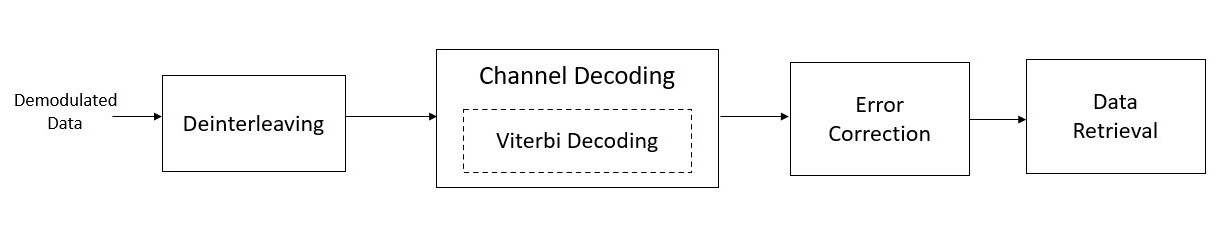
\includegraphics[width=1.2\columnwidth]{figs/decoding_r}
\centering
\captionsetup{justification=centering}
\caption{The Block Level Architecture for Channel decoding}
\label{fig:decoding_r}
\end{figure}
\end{normalsize}


\subsection{Maximum Likelihood Decoding}
The first 52 bits of the frame are a part of subframe 1 and are BCH encoded. To decode these bits, we use a modified version of ML decoding. Before encoding, subframe 1 has 9 bits. These 9 bits give us the TOI (Time of Interval) data. The TOI for NavIC L1 ranges from 1 (000000001) to 400 (110010000). After encoding, SF1 will have 52 symbols. So there will be 400 possible combinations of SF1 before and after encoding. 

So, on the receiving side, we generate these 400 possible codewords and keep them in a lookup table. When a frame is received, the first 52 symbols are separated. The received codeword is compared with every other codeword in the loookup table and the hamming distance is calculated. The codeword in the lookup table which has the least hamming distance with the received codeword is the  corrected codeword (NOTE: Works only if error < 20 bits. This method fails for very noisy channels). The corresponding bit sequence (decoded) can be mapped from the chosen codeword.

\subsection{Deinterleaving}
To reduce the burst error while transimission, the LDPC encoded symbols are interleaved into a 38x46 matrix. Data is written in columns and then, read in rows. So even if there is any burst error, it is spread out. At the receiving side, the matrix is then converted to a regular row of symbols.

\subsection{Belief Propagation}
The basic concept of the algorithm involves message passing. Messages are passed iteratively between adjacent nodes until convergence dictated maximal number of iterations. The nature of the messages involves probabilities or log-likelihoods of probabilities. As nodes receive messages from their nearest neighbors, they improve their estimate regarding received bits. For sufficiently long blocks, with sufficiently long cycles, the algorithm has been shown empirically to perform well.

Variable nodes pass messages that involve the log-likelihood of some bit being 0 or 1 by processing information obtained from other check nodes and the channel whereas check nodes pass messages which involve the log-likelihood of a parity equation is satisfied by processing information obtained from other variable nodes.

For each node of the factor graph, there are two directions of soft information in the form of LLR. The LLR propagated from right to left is denoted as $L_{i,j}$, while that from left to right is denoted as $R_{i,j}$. The decoder employs the so-called processing element (PE), which performs the following LLR estimations with the Min-Sum approximation, so that LLRs are traversed through the factor graph.

BPD is performed on the factor graph by operating the PE from left to right, and from right to left to update L and R, respectively. The final decision is estimated after the completion of all the  iterations. After decoding, CRC is calculated to verify the decoded data.









